  \section{Conclusiones}

    Para determinar la ecuación de cálculo del ángulo de desfasaje, a partir 
    de la figura de Lissajous se debe tener en cuenta que

    \begin{align*}
      f(t)=A \cdot sen(\omega \cdot t + \phi) \hspace{20pt} \land \hspace{20pt} g(t)=A \cdot sen(\omega \cdot t),
    \end{align*}

    donde g(t) es la referencia, y se coloca en el eje x de la figura por convención y
    cada punto de la Figura de Lissajous se compone en coordenadas

    \begin{align*}
     Lissajous(X,Y)= ( \hspace{5pt} g(t) \hspace{10pt} ; \hspace{10pt} f(t) \hspace{5pt}).
    \end{align*}
    
    Si se hace $t=0$, entonces $g(t)=0$, y 

    \begin{align*}
      f(0)=A \cdot sen(\phi) \hspace{20pt} \Longrightarrow \hspace{20pt} \Aboxed{sen(\phi)=\frac{f(0)}{A}}.
    \end{align*}

    En la figura de Lissajous, f(0) se corresponde con el corte del trazo con el eje vertical, y A es el valor 
    máximo absoluto que alcanza la señal.

    Luego por trigonometría se puede deducir que:

    \begin{align*}
      sen^2(\phi)+cos^2(\phi)=1 \hspace{20pt} \Longrightarrow \hspace{20pt} \Aboxed{cos(\phi)= \sqrt{1 +  \left( \dfrac{f(0)}{A} \right)^2} }.
    \end{align*}

        \begin{figure}[H]
          \centering
            \frame{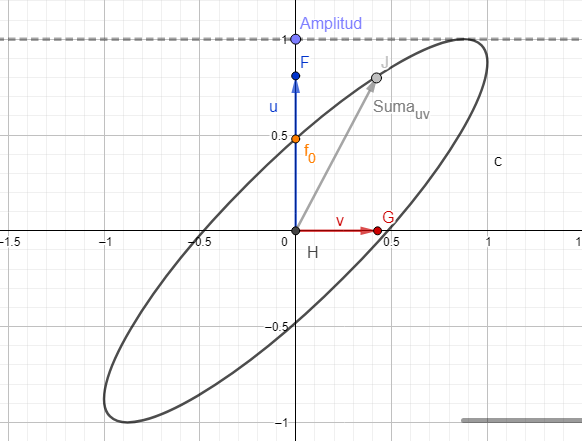
\includegraphics[width=0.7\textwidth]{Imagenes/Conclusiones/Figura_Lissajous_Geo.png}}
            \caption{Curva Lissajous.}
            \label{fig:Lissajous}
        \end{figure}

    Para determinar la ecuación del cálculo del capacitor de compensación se parte de la siguiente
    premisa:

    \begin{align*}
      I_{Xc} = I \cdot sen(\phi) \hspace{20pt},
    \end{align*}

    donde $I_{Xc}$ es la corriente reactiva debido al capacitor, I la corriente total y $\phi$ el 
    ángulo de desfasaje entre la tensión y corriente, el cual se quiere corregir.

    Dividiendo ambos miembros por la tensión V total, se tiene

    \begin{align*}
       \frac{I_{Xc}}{V} = \frac{I \cdot sen(\phi)}{V} \hspace{20pt},
    \end{align*}

    recordando además la ecuación de Reactancia de un capacitor que es

    \begin{align*}
        Xc = \frac{V}{I_{Xc}} = \frac{1}{\omega \cdot C} \hspace{20pt},   
    \end{align*}

    se tiene entonces que

    \begin{align*}
       \frac{1}{Xc} = \omega \cdot C = \frac{I \cdot sen(\phi)}{V} \hspace{20pt}.
    \end{align*}

    Usando la relación de potencia aparente se reemplaza I obteniéndose 

    \begin{align*}
      \omega \cdot C = \frac{S \cdot sen(\phi)}{V^2} \hspace{20pt},
    \end{align*}

    por último multiplicando y dividiendo el segundo término por $cos(\phi)$ y despejando C

    \begin{align*}
       \omega \cdot C = \frac{ \frac{S \cdot cos(\phi) \cdot sen(\phi)}{cos(\phi)}}{V^2}\hspace{20pt} \Longrightarrow \hspace{20pt} \Aboxed{C = \frac{P \cdot tg(\phi)}{\omega \cdot V^2}}\ .
    \end{align*}

    Se ha visto a lo largo del presente informe que el agregado del capacitor de corrección produce
    una deformación en la onda de salida del resistor R1, debido a la propiedad de los capacitores de 
    realce de alta frecuencia, con lo que el ruido montado en la señal se ve amplificado.
    

    
